\chapter{Introduction}
\label{Chapter1}
\settocdepth{subsection}
Image edge detection and image segmentation are key problems in computer vision.
%While the two problems are related

\section{Motivation}
% Recently, very good edge detection results were achieved using random decision forests \cite{DollarICCV13edges}.
In recent years innovative approaches have lead to significant advances %improvements for 
in the task of {\bf edge detection}. 
While a certain edge model is imperative, % required, needed % a requirement
few segmentation algorithms rely on edge information %make use of edge detection output 
as a first step towards %to 
{\bf image segmentation}. Consequently, many edge detection algorithms re-use the same approach to obtain image segmentation in addition %additionally 
to their edge detection output.

Therefore, the field of image segmentation is limited by lack of research on hierarchical segmentation methods which are based on edge detection output. % edge-based hierarchical segmentation. 
We investigate a technique % possibility 
to obtain image segmentation given an edge detector output, which is an alternative to a currently popular % widely-used  
method. We propose a principled solution that uses the inherent structure and context from local patches. We utilise that to grade the salience of region boundaries - a prerequisite for a multiscale segmentation.

\section{Problem definition}
We address the problem of generic % or general? 
image segmentation. To help understand it, it is necessary to first introduce the notions of an {\it edge} - an essential for edge detection, and {\it contour} - a requirement for image segmentation.

% TODO is the field young? here, I meant more boundary detection and general image segmentation, which came to add new terminology, but here it's too early to go into details
\textbf{Terminology:} % As the field is young, it 
It is worth pointing out that there is a certain lack of consistency and differences in definitions as concerns related terminology. In the following we define the basic vocabulary for our method and we will be consistent in using it throughout this report.

\subsection{Edge detection}
%- (from Maire thesis)
% Contours  convey  key  information  about  object  shape  and  serve  as  the  basis  for  a variety of local image descriptors, such as SIFT[Lowe, 1999], shape context[Belongie et al., 2002], and geometric blur[Berg and Malik, 2001], used in recognition systems.Hence,  improvements at the contour detection stage can impact the quality of the descriptors used in a wide range of vision algorithms
Image edges carry crucial % , central, essential, indispensable, pivotal, critical, dominant, vital, principal, prime, primary, chief, major, leading, main, important, significant, key 
information about object shape. The extraction of edges from digital images has its application in %tasks such as 
object detection and recognition, segmentation, structure from motion, and tracking. Further, edges are basis for a number of local descriptors, \eg SIFT \cite{Lowe1999object,Lowe2004distinctive}, shape context \cite{Belongie2006matching}, HOG \cite{Dalal2005histograms}.

% TODO use a horizontal image as example, will fit two at a line without taking so much space
\begin{figure}[ht!]
\centering
 \subfigure[Input image from %the validation subset of 
 BSDS500~\cite{BSDS500resources}]{%
  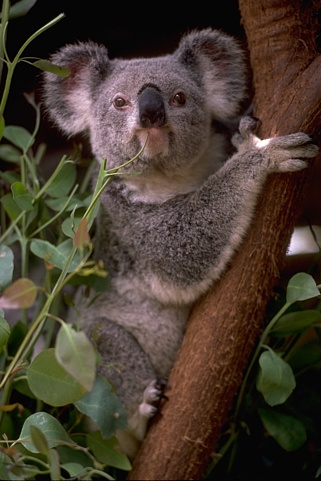
\includegraphics[width=0.35\textwidth]{images/examples/koala/koala.jpg} % hawaii/arbelaez2011-035.png}
 }
 \subfigure[Edge map]{%
  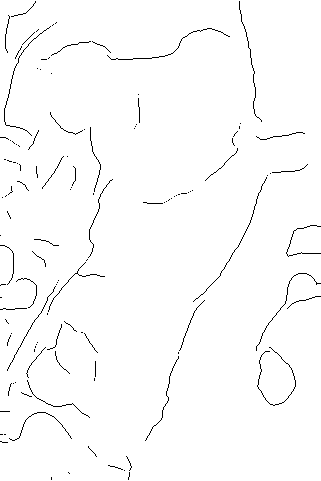
\includegraphics[width=0.35\textwidth,frame]{images/examples/koala/koala_gPb_edge_map.png} % too thin - SE are thicker koala_SE_edge_map % hawaii/edge_map_arbelaez2011-039.png}
  \label{fig:sub:edge_detection-edge-map}
 }

 \subfigure[Probability of boundary ({\bf Pb})]{%
  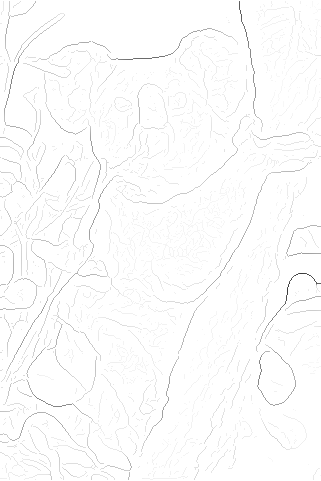
\includegraphics[width=0.35\textwidth,frame]{images/examples/koala/koala_gPb.png} % koala_SE % hawaii/Pb_arbelaez2011-039.png}
  \label{fig:sub:edge_detection-pb}
 }
 \subfigure[{\bf Pb}, colour-coded]{%
  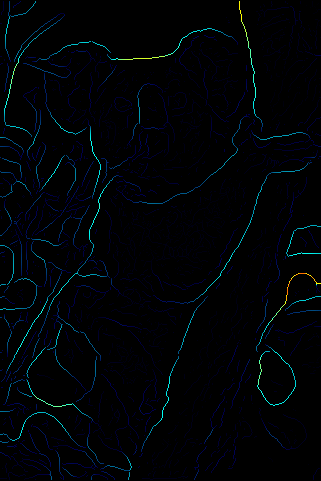
\includegraphics[width=0.35\textwidth]{images/examples/koala/koala_gPb_cc.png} % koala_SE_cc % hawaii/Pb_arbelaez2011-039.png}
  \label{fig:sub:edge_detection-pb-cc}
 }
\caption[Edge detection - edge map and probability of boundary]{{\bf Edge detection}. Note that for ease of view, % for illustrative purposes % illustration
the negative of \protect\subref{fig:sub:edge_detection-edge-map} and \protect\subref{fig:sub:edge_detection-pb} are shown, \ie the darker the pixel, the higher the probability of an edge. Visualisation code for \protect\subref{fig:sub:edge_detection-pb-cc} courtesy of Hallman and Fowlkes~\cite{Hallman2014}.}
\label{fig:edge_detection}
\end{figure}

\subsubsection{Edge, edge map, probability of boundary}
\paragraph{Image edge}\mbox{}\\\mbox{}\\
Image edge detection deals with the problem of finding pixels which belong to object boundaries within a digital image. Those %The pixels belonging to object boundaries in an image are often locations 
often, but not always, coincide with image locations where a sharp change of image brightness occurs. Those locations of image intensity discontinuities are called \textit{image edges}. Due to the properties of natural images, edge pixels in them are typically grouped together. 

\paragraph{Edge map}\mbox{}\\\mbox{}\\
We will call an \textit{edge map} a binary image $M$ depicting edges' locations. The pixels belonging to an edge are set to 1. The rest of the pixels are not part of an edge. They have a value of 0. Therefore, for a given pixel location $(x,y)$, the corresponding edge map value is $M_{(x,y)} \in \{0,1\}$ (see \fref{fig:sub:edge_detection-edge-map}).

% from \cite{Shi2000normalized}
%- A Bayesian view is appropriate - there  are  several  possible  interpretations  in the  context of prior  world  knowledge.  The  difficulty,  of course, is in specifying the prior world knowledge. Some of it  is  low  level,  such  as  coherence  of  brightness,  colour,texture,  or  motion,  but  equally  important  is  mid-  or  high-level   knowledge   about   symmetries   of   objects   or   object models.

\paragraph{Probability of boundary}\mbox{}\\\mbox{}\\
To allow to express a level of (un)certainty as to the presence of an edge in an image, we employ a probabilistic means. We define a real-valued image $Pb$, which stands for \textit{Probability of boundary} (see Figures \ref{fig:sub:edge_detection-pb} and \ref{fig:sub:edge_detection-pb-cc}). For a given pixel location $(x,y)$, the corresponding value is $Pb_{(x,y)} \in [0,1]$.

The Bayesian view of edge detection as a posterior probability given prior world knowledge is not new. %The notion of probability of a location being a boundary %an edge 
% pixel was first introduced in \cite{Martin2004learning}. % TODO really?
This particular definition of {\it Pb} was, to our knowledge, first introduced in \cite{Martin2004learning} with the development of the detector with the same name {\tt Pb} ({\it MFM (Martin-Fowlkes-Malik)} in the paper). It has ever since been used as an output for %to 
many edge detection algorithms \cite{Arbelaez2006boundary,Dollar2006supervised,Maire2008using,LimZD13,DollarICCV13edges,Isola2014crisp,Ganin2014n4fields,Hallman2014} as it combines nicely with the boundary evaluation methodology, also proposed in \cite{Martin2004learning}.

\paragraph{Thresholding}\mbox{}\\\mbox{}\\
Given a {\it Pb}, we can obtain edge maps at different levels of detail by {\it thresholding}. We choose a threshold $t\in(0,1)$ and consider as detected edge pixels those locations $(x,y)$ for which it holds %such that 
$Pb(x,y)>t$. Obviously, a lower threshold allows to discover more edges, while a higher threshold is more conservative and would only honour the most salient of edges.

\paragraph{Example}\mbox{}\\\mbox{}\\
In \fref{fig:edge_detection} we show the result of the edge detection algorithm {\tt gPb} \cite{Arbelaez11}, which we will describe in more detail in \cref{Chapter3}.

The last two images display the detector output - a {\it Pb}. For improved viewing in case of probabilistic output we will utilise a visualisation with black as background and heatmap-coloured boundaries according to their strength. This visualisation of probabilistic output facilitates the qualitative comparison of the results of different algorithms. 

The {\it edge map} in \fref{fig:sub:edge_detection-edge-map} was obtained by thresholding at $t=0.3$ the {\it Pb} from \fref{fig:sub:edge_detection-pb}.

\subsection{Image segmentation}
One of the main principles of Gestalt psychology concerns the human visual system \cite{Wertheimer1923untersuchungen,Kohler1929task,Koffka1935principles,Wertheimer1938laws}. Our ability to organise our visual input and perceive objects and prominent parts of objects is termed {\it visual grouping}. 

Image segmentation is the computer vision attempt at scientific study and imitation of this phenomenon. It is the task of partitioning a digital image into meaningful parts. Those parts, called {\bf segments}, should unify homogeneous (\wrt colour or texture) % is there a need to be homogeneous
regions which correspond to objects, parts of objects, or background. The purpose of this decomposition is to ease further analysis by substituting reasoning on the \textit{\textbf{superpixels}} (another term for ``segments'') {\it graph} for reasoning on the {\it pixels grid}. % substitute _ for _: ``Industry must reduce fuel consumption by substituting alternative fuels for fossil fuels.''

\begin{figure}[ht]
\centering
 \subfigure[Input image]{%
  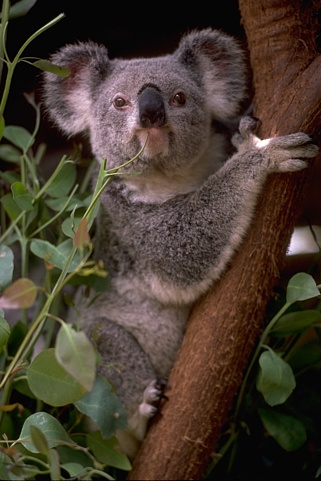
\includegraphics[width=0.1\textwidth]{images/examples/koala/koala.jpg}
 }
 \subfigure[Segmentation - {\bf labelling}]{ % (implicit boundary)]{%
  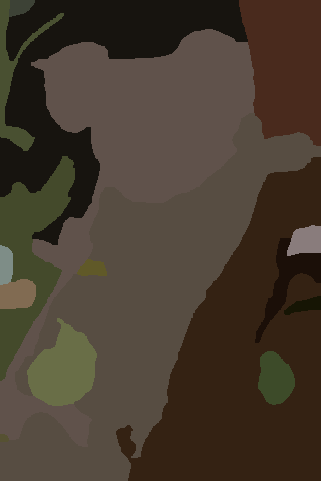
\includegraphics[width=0.2\textwidth]{images/examples/koala/koala_segm_labelling.png}
  \label{fig:sub:segmentation-segm-labelling}
 }
 \subfigure[{\bf Region}]{ %, segment, superpixel
  
\includegraphics[width=0.2\textwidth,frame]{images/examples/koala/koala_gPb_region.png}
  \label{fig:sub:segmentation-region}
 }
 \subfigure[Region boundary - a {\bf contour}]{%
  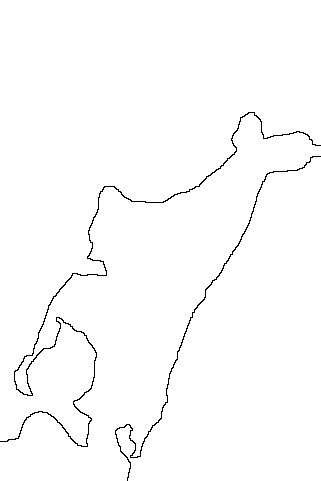
\includegraphics[width=0.2\textwidth,frame]{images/examples/koala/koala_gPb_region_bdry.png}
  \label{fig:sub:segmentation-region-contour}
 }
 \subfigure[Segmentation {\bf contours} of \protect\subref{fig:sub:segmentation-segm-labelling} and \protect\subref{fig:sub:segmentation-segm-explicit}]{%
  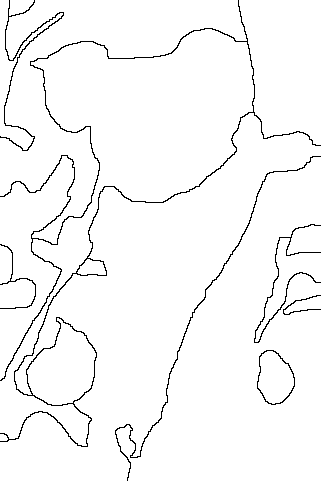
\includegraphics[width=0.2\textwidth,frame]{images/examples/koala/koala_segm_bdry.png}
  \label{fig:sub:segmentation-segm-bdry}
 }
  \subfigure[Segmentation - {\bf explicit contour}]{%
  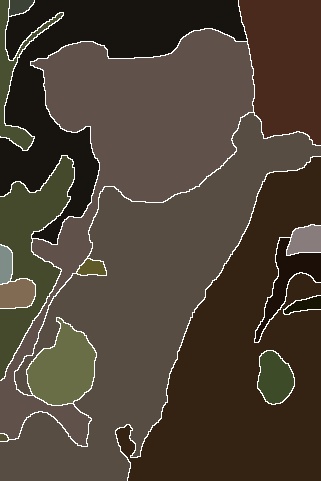
\includegraphics[width=0.2\textwidth]{images/examples/koala/koala_segm_explicit.png}
  \label{fig:sub:segmentation-segm-explicit}
 }
 \subfigure[Hierarchical segmentation - a {\tt UCM}~\cite{Arbelaez2006boundary}]{%
  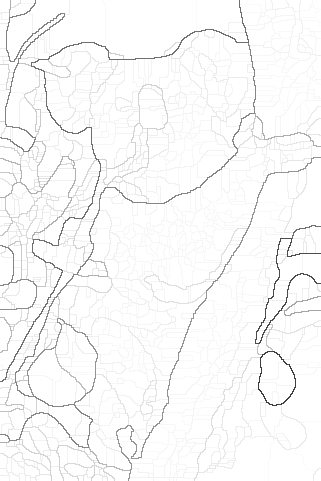
\includegraphics[width=0.35\textwidth,frame]{images/examples/koala/koala_ucm.png}
  \label{fig:sub:segmentation-ucm}
 }
 \subfigure[{\tt UCM}, colour-coded]{%
  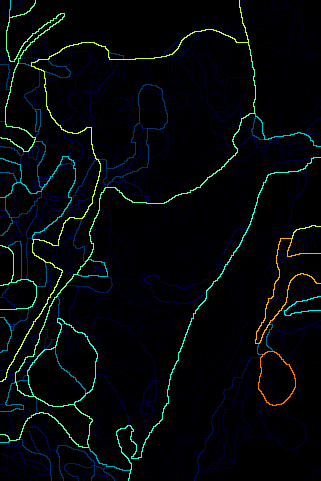
\includegraphics[width=0.35\textwidth]{images/examples/koala/koala_ucm_cc.png}
  \label{fig:sub:segmentation-ucm-cc}
 }
\caption[Image segmentation - segmentation, contour, region, hierarchical segmentation]{{\bf Image segmentation}. As in \fref{fig:edge_detection}, we show the negative of the probabilistic output. For segmentations we use the mean pixel colour from the image to represent the whole segment. The {\tt UCM}s are enlarged to make details easier to discern.}
\label{fig:segmentation}
\end{figure}

\subsubsection{Contour, segmentation, region boundary, hierarchical segmentation}
\label{sec:ch1-segmentation-terminology}
\paragraph{Image segmentation}\mbox{}\\\mbox{}\\
As already mentioned, a {\it segmentation} of a digital image is a partition of it into a set of distinct {\it segments} (also known as {\it regions}, or {\it superpixels}).

When we visualise a segmentation each region will be depicted by the mean colour value (from the original image) of all the pixels that are part of it, %by its {\bf mean colour} 
as in \fref{fig:sub:segmentation-segm-labelling}.

\subparagraph{Segmentation labelling}\mbox{}\\\mbox{}\\
In practice, we will call {\it segmentation labelling} a labelling of each pixel in the image, such that two pixels have the same label if and only if %iff 
they belong to the same region. No two regions should have the same label. Uniqueness of segmentations is defined up to a permutation of the labels. 

\paragraph{Region}\mbox{}\\\mbox{}\\
Regions (also {\it segments}, or {\it superpixels}) are the building blocks of a segmentation. The outline %boundary 
of a region fulfils the definition for an {\it image edge}. What is more, it constitutes a {\bf closed boundary}, which we will call {\bf contour}. See Figures \ref{fig:sub:segmentation-region} and \ref{fig:sub:segmentation-region-contour}.

\paragraph{Segmentation contours}\mbox{}\\\mbox{}\\
Note that it is {\it sufficiently easy} (further explanation to be given shortly) to obtain an {\bf edge map} from a segmentation - one just has to consider all the outlines of all the regions % superpixels
(the boundaries between the segments). The resulting edge map (\fref{fig:sub:segmentation-segm-bdry}) has the added benefit that all edges are in fact closed - they are {\bf contours}.

\paragraph{Segmentation represented with explicit contours}\mbox{}\\\mbox{}\\
So it is plain to see that there exists a {\bf duality between segmentation regions and contours}, in that the superpixels enclosed by the contours constitute % do %would form 
the segmentation regions. 

If we think of the task of {\bf manually annotating the segmentation} of an image, we will notice that hand-drawing the contours delineating the objects is easier than hand-labelling each pixel according to %based on 
its region membership. It is more natural, therefore, to first mark %have 
the segmentation contours, and have them determine the regions - see \fref{fig:sub:segmentation-segm-explicit} for an example of a segmentation with explicit boundary. 

In this case obtaining the {\bf segmentation contours} is trivial - we just take the explicit region boundaries (and mark the pixels internal to the regions as ``background'', with an edge map value of 0). Thus we have obtained an {\bf edge map}, as in \fref{fig:sub:segmentation-segm-bdry}.

\paragraph{Segmentation contours from segmentation labelling}\mbox{}\\\mbox{}\\
In case of segmentation represented by labelling (\fref{fig:sub:segmentation-segm-labelling}), \ie~{\bf implicit boundary} between the regions, care must be taken in order to obtain the contours. The trouble lies in the fact that there is an ambiguity as to the correct placement of the boundaries (if the resulting edge map image should be with the same resolution). A possible solution is the use of {\it super-resolution}, which means doubling the resolution of the image and placing the boundaries in between the segment labels. Other solutions that do not change the image %stay on the same 
resolution should be consistent in how exactly they place the %placement of 
boundaries when converting between the two representations.

\textbf{Both segmentation representations are important to us:} In the rest of this report, more specifically in \cref{Chapter4} (which describes our algorithm) and \cref{Chapter5} (which accommodates our experiments), we will make use of both representations - labelling and explicit contours - for segmentation. % EDIT (Mathieu) both representations for segmentation - labelling and explicit contours. %boundaries.

\paragraph{Hierarchical segmentation}\mbox{}\\\mbox{}\\
\textbf{Encoding the saliency of region boundaries:} For the problem of edge detection {\it Pb} allows to encode the {\bf degree of confidence} as to the presence of an edge. It would be convenient to have a similar means for the task of image segmentation. 

\textbf{Over- and undersegmentation:} If segmentation splits up the image into too many regions, it is termed an {\it oversegmentation}, and if they are too few (\eg a segment contains more than one object) - an {\it undersegmentation}. In addition to the above demand, % requirement
we would like to be able to obtain segmentations at {\bf different levels of detail} - on the full scale from an oversegmentation to an undersegmentation. 

Both requirements are %That is 
easily satisfiable by using a data structure called an {\it Ultrametric contour map} ({\tt UCM}) \cite{Arbelaez2006boundary}. While details will be given in \sref{sec:ch3-UCM}, for now it is sufficient to know that it represents %encapsulates 
a hierarchy of segmentations. 
Like with {\it Pb}, {\bf thresholding} the {\tt UCM} allows to obtain a segmentation.

Note that the idea of controlling the coarseness of a segmentation by using a multiscale segmentation is not new \cite{Sharon2000fast,Sharon2001segmentation,Galun2003texture}. %, and get at each scale a level of detail(?s?) compatible with the perceptual organisation of the image at this scale. 
{\tt UCM} is just one means of encompassing a hierarchy of segmentations at different scales. 
As we will see in \sref{sec:ch3-UCM}, it is particularly suitable for us as a last stage of a segmentation pipeline which starts with extraction of edges.

\paragraph{Example}\mbox{}\\\mbox{}\\
In \fref{fig:segmentation} we show the result of the algorithm {\tt gPb-OWT-UCM} \cite{Arbelaez09,Arbelaez11}, which we will present in \cref{Chapter3}. The output is a {\tt UCM} - see \fref{fig:sub:segmentation-ucm} for an example of {\tt UCM} output and \fref{fig:sub:segmentation-ucm-cc} for its colour-coded visualisation.

The segmentation in Figures \ref{fig:sub:segmentation-segm-labelling} and \ref{fig:sub:segmentation-segm-explicit} was obtained by thresholding the {\tt UCM} at $t=0.4$.

\settocdepth{section}
\subsection{Problem statement}
Our task in the present work is to perform {\bf generic image segmentation}. More specifically, we would like to do segmentation, basing ourselves off the output of an edge detector - the % NOTE posterior (?) % <- it is posterior in the case of gPb, after they do all the magic with their cue combination (Pb), sPb, and mPb
{\it Pb}: a probability of an edge for each pixel location.

\subsection{Challenges}
\label{sec:ch1-problem-challenges}
There is a %general 
consensus in the research community \cite{Martin2004learning} that {\bf general edge detection} is, up to a point, % a bit, to some extent, (up) to a point, in some measure, rather (- somewhat) 
ill-defined % dubious 
in the sense that it is not clear what {\it universally} determines %defines 
a correct output. The measure of detail is both subjective and application-specific. % (up to the person)

The same pertains to % concerns
{\bf general image segmentation}, since the quality and utility of the obtained segments are task-dependent. % a.k.a. application-specific 
Hence, with {\it general} segmentation, there is an ambiguity as to the correct level of granularity of %on 
the ground truth segments. % admissible, valid
Different people would perform different acceptable segmentations. This is exhibited in datasets containing images (BSDS500 \cite{BSDS500resources}) and videos (VSB100 \cite{Galasso13}) with {\it multiple annotations} per entity. The average human agreement tends to be approximately 80-90\%. 
Typically, %human 
subjects would concur on the most salient objects in the scene and disagree on secondary and\slash or background ones.
%Typically, subjects would agree on the most salient objects in the scene and differ on secondary and\slash or background ones.

\subsection{Remark about %Confusion with 
semantic segmentation}
\settocdepth{subsection}
The segments discovered by {\bf generic image segmentation} should be {\it meaningful} in a higher-level sense - when not background, they should be objects, or prominent parts of objects. Therefore the regions in the segmentation should respect, \ie not cross, boundaries of objects.

The term {\bf semantic segmentation}, however, has come to be associated in the computer vision community with a different task. The goal of semantic segmentation is the automatic labelling of image regions and pixels with category names. Also, the machine %it 
is expected to segment an image into a {\it small number} of significant %meaningful 
regions with {\it considerable size}, see \fref{fig:semantic-segmentation}. Semantic segmentation serves the purposes of %is applied for 
scene understanding and semantic interpretation of images.

\begin{figure}[ht!]
 \centering
 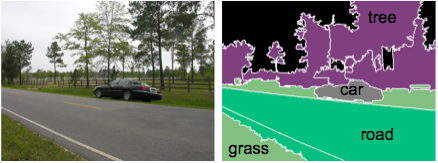
\includegraphics[width=0.51\textwidth]{images/intro/semantic-segmentation.png}
 \caption[Semantic segmentation]{Semantic segmentation requires segments to be assigned to designated %pre-defined 
 categories. Courtesy of \cite{VisualLearningTutorial2013}.}
 \label{fig:semantic-segmentation}
\end{figure}

A commonality % similarity 
with general segmentation is the fact that different people are still likely to draw different segmentation results for the same image because their semantic interpretations differ. One should keep in mind, however, that semantic segmentation %it 
aims for the pixel-wise {\it classification} of images, and to this end %it 
makes use of predefined categories.

The two flavours of image segmentation tasks should not be confused. In this paper we work on {\bf general segmentation}.

\section{Related work}
\subsection{Edge detection}
Early edge detection approaches solely rely on local cues. Low-level detectors define edges as sharp discontinuities in image brightness. First results were achieved using digital image processing techniques. The {\bf Roberts cross} \cite{Roberts1963machine}, {\bf Sobel filter} \cite{Sobel19683x3}, and {\bf Prewitt operator} \cite{Prewitt1970object} all are discrete differentiation operators. % can say 'differential operator'
They view an image as a 2-dimensional signal which they convolve with pre-defined filters with local support. In the same line of work is the {\bf Marr-Hildreth} algorithm \cite{Marr1980theory}, which finds zero-crossings of the Laplacian of the image intensity. Later still, the {\bf Canny detector} \cite{Canny1986computational} produces %shows 
better-quality edges. It searches for extrema in the gradient of the image intensity. % EDIT (Mathieu) for peak gradient magnitude in the image intensity. 
It introduces %adds some 
improvements, like {\bf non-maximum suppression} (also known as ``edge thinning''), which refines %improves 
edge localisation. A practically relevant extension is the {\bf Canny-Deriche detector} \cite{Deriche1987using}, which addresses the filter implementation of the Canny operator.

The presence of noise, clutter, texture, and non-homogeneous object parts interfere with % hamper, hinder, impede 
the effectiveness of the above detectors. Higher-level techniques incorporate colour and texture \cite{Rubner1996coalescing,Will2000learning,Malik2001contour} information, as well as multiple scales \cite{Martin2004learning} and orientations \cite{Perona1990detecting,Freeman1991design}.

Globalisation could be added \cite{Maire2008using,Xiaofeng2012discriminatively} to improve accuracy by focusing on the most salient edges.

% TODO this paragraph - focus
%- edge - Abrupt change in some low �level image feature such as brightness or colour
%- boundary - Contour in image plane that represents a change in pixel ownership from one object to another 
Yet higher quality edge detection is desirable. Texture edges and illusory contours are elusive to % escape from
traditional edge-detection algorithms. Recent approaches therefore rely on {\bf learning} to incorporate context and object knowledge. They address more challenging scenarios which arise in natural images. 

As Martin \etal argue in \cite{Martin2004learning}, such methods solve the so-called ``boundary detection'' problem. A {\bf boundary} delineates the pixels that belong to one object, material, or surface from those that belong to another. One possible approach to boundary detection is to go top-down and use higher-level object knowledge to infer the object boundaries. Another solution would be to use edges as low-level cues to judge for the presence of object boundaries (a bottom-up approach). This is how Martin \etal tackle the problem in their {\tt Pb} detector and its subsequent development - {\tt gPb} \cite{Maire2008using} (see next).

% TODO what did I mean by that? SE and gPb ARE general edge detectors and are quite adequate
% In such more challenging situations a \textit{general} edge detector would not be adequate, since the desired output is application-specific.

\subsubsection{Current state-of-the-art edge detectors}
\paragraph{{\tt gPb}:} {\tt gPb} (for {\it global probability of boundary}) \cite{Martin2004learning,Maire2008using} is a popular edge detector; we employed it earlier in the chapter for the illustration of edge-related terminology (in \fref{fig:edge_detection}). It works by extracting features from a local patch and estimating the posterior probability for an edge through the centre of the patch. Multiple scales and globalisation based on a spectral clustering framework % Normalised Cuts 
help achieve high-quality results. We review {\tt gPb} in \sref{sec:ch3-gPb}.

\paragraph{Structured edge:} The {\it structured edge} ({\tt SE}) algorithm \cite{DollarICCV13edges,Dollar2015PAMI} utilises supervised learning to train a structured decision forest. The trained forest ``knows'' edge structure from local image patches, and can predict the most likely segmentation patch for an unseen patch. We dissect this work in \cref{Chapter2}.

\paragraph{\texorpdfstring{$N^4$}{N4}-Fields:} The {\tt N4-Fields}, for {\it neural network nearest neighbour} \cite{Ganin2014n4fields} presents the first state-of-the-art results for natural edge detection obtained with deep learning. It applies {\it convolutional neural networks} ({tt CNN}s, or {\tt ConvNet}s) \cite{Fukushima1980neocognitron,Lecun1998gradient} jointly with {\it nearest-neighbour} search.

\paragraph{Crisp boundary detection using \textit{pointwise mutual information} ({\tt PMI}):} The method, due to Isola \etal \cite{Isola2014crisp}, utilises internal image statistics to model the presence of an edge. It derives an affinity measure from {\tt PMI}, which is a good predictor of whether or not two pixels reside on the same object. The authors then reuse the spectral partitioning machinery which is part of the {\tt gPb} algorithm (to be explained in \sref{sec:ch3-sPb}). The method produces 
{\it crisp} edges, \ie of pixel-level accuracy.
% pixel-level accurate (\ie {\it crisp}) edges. %boundaries.

\paragraph{Oriented edge forests ({\tt OEF}):} In their recent work \cite{Hallman2014}, Hallman and Fowlkes use a random forest classifier for edge patches. They limit the algorithm to only straight-line edges of a fixed number of positions and orientations. A post-processing sharpening of the edge masks boosts edge localisation accuracy. We briefly discuss this work as a good means of capturing local context in \sref{sec:ch2-alternative-capturing-context}.

\subsection{Image segmentation}
Image segmentation is a 
% difficult %complex 
% problem that has received lots of research in the past. 
longstanding and difficult computer vision research problem.
Many segmentation techniques have been developed, but each has its weaknesses and limitations. It is therefore currently not easy to select %choose 
a universally best {\it general segmentation} method.
%- A universal algorithm for segmenting images certainly does not exist and, on the contrary, most techniques are tailored on particular applications and may work under certain hypothesis.

The following is by no means a comprehensive survey of image segmentation algorithms, as the problem is old and there exist many and varied approaches to solving it. Instead, it provides 
a selection of methods (a) highly relevant to our proposed approach, and\slash or (b) the current state-of-the-art. 
% a selection of 1) highly relevant to our proposed approach, and\slash or 2) current state-of-the art methods.
% NOTE more: a) variational framework (Mumford and Shah) - energy minimisation; b) Chan and Vese - ``level set'' formalism; c) convex relaxation of a)

\subsubsection{Watershed transformation} % TODO transformation or transform?
\label{sec:ch1-watershed-transform}
The watershed transformation is a basic morphological operation \cite{Beucher1992morphological} used to produce an image segmentation. We review it in detail in \sref{sec:ch3-watershed}, as it is part of the segmentation pipeline that we propose. A major problem with using it as a general segmentation algorithm is its inherent % intrinsic 
tendency oversegment natural images. %to produce oversegmentations from natural images.

\subsubsection{Region growing}
The {\bf seeded} region growing algorithm \cite{Adams1994seeded} takes as input the image and a set of seeds. The seeds mark each of the target objects to be segmented. The regions are iteratively grown by comparing the regions to the unallocated pixels that border them. This method is much dependent on the order in which the unallocated pixels are examined, and the choice of seeds for the regions. Manual choice of seeds is undesirable % inconvenient
and image noise can result in their poor automatic placement.

{\bf Unseeded} region growing \cite{Lin2000unseeded} was subsequently developed, which uses the Perona-Malik anisotropic diffusion \cite{Perona1990scale}. It allows to forgo the choice of seeds (only one is required to mark a first region), and other regions are ``discovered'' in the process of segmentation. However, this algorithm exhibits a bias towards growing earlier discovered regions.

Proper choice of parameters remains a problem for both methods.

\subsubsection{Region merging}
% TODO give any difference and comparison between those
This method divides the image into many small regions. 
% Adjacent regions are merged together if %in case 
% certain criteria (\eg allowed colour ranges, minimum\slash maximum size of a region) are met. 
Adjacent regions are merged together based on their {\it spatial} (compactness and smoothness of region) and {\it spectral} (variance of colour within a region) heterogeneity. 
The process continues until no regions meet the merging criteria. Region merging algorithm implementations differ in their merging predicate (\eg allowed colour ranges, minimum\slash maximum size of a region) and the order of the merges. 

\paragraph{Felzenszwalb and Huttenlocher's algorithm}\mbox{}\\\mbox{}\\
% from \cite{Arbelaez09}
%- Felzenszwalb and Huttenlocher[15] is typically used in high recall settings to create a gross oversegmentation into thousands of superpixels
A prominent example of region merging is the method developed %invented 
by Felzenszwalb and Huttenlocher ({\tt Felz-Hutt}) \cite{Felzenszwalb1998ciently,Felzenszwalb1998image,Felzenszwalb04}. This graph-based segmentation algorithm is a {\bf greedy region merge} whereby the notion of an {\bf image edge} evidence is encoded implicitly as a pairwise pixel constraint.

\paragraph{Statistical region merging}\mbox{}\\\mbox{}\\
Another well-known region merging implementation is {\tt Statistical region merging} \cite{Nock2004statistical}.

\subsubsection{Normalised cuts}
%- from \cite{Arbelaez09}
% Mean Shift and Normalised Cuts provide better precision, but often produce artefacts by breaking large uniform regions (e.g.sky) into chunks.
The {\it normalised cuts} ({\tt N-Cuts})
algorithm \cite{Shi2000normalized} casts the segmentation problem as a partitioning problem on the image pixel graph. This is further reduced to a spectral clustering (generalised eigenvalue) problem, effectively allowing the method to make decisions based on global properties of the input.

\subsubsection{Mean shift}
The {\tt Mean Shift} method of Comaniciu and Meer \cite{Comaniciu2002mean} is a non-parametric mode-finding technique that is applied on clusters in feature space. The algorithm, along with {\tt N-Cuts}, is remarked \cite{Arbelaez09} to produce artefacts by breaking large uniform regions (\eg sky, grass), due to a normalisation for the size of the segments. % TODO check if this is really the reason

% from \cite{Nock2004statistical}
%-  A prominent trend in grouping focuses on graph cuts, mapping image pixels onto graph vertices, and the spatial relationships between pixels onto weighted graph edges. The objective is to minimize a cut criterion, given that any cut on this graph yields a partition of the image into(hopefully) coherent visual patterns. Cut criteria range from conventional [2] to more sophisticated criteria, tailored to grouping [3], [4], [5]. These are basically global criteria;however, the strategies adopted for their minimization range through a broad spectrum, from local [6] to global optimisation [5], through intermediate choices [7], [3]. Global optimization strategies have the advantage to directly tackle the problem as a whole, and may offer good approximations[5], at possible algorithmic expenses though [3], [5].

%- Among these schemes,three methods have proven to be quite popular in practice owing to their performance and/or their running time.  The Mean Shift method of Comaniciu and Meer [6],  the Normalized Cuts method developed by Shi and Malik [14] and the graph based method of Felzenszwalb and Huttenlocher

%- More  Recently  Arbelaez,  Maire,  Fowlkes  and  Malik[3, 2] have proposed an impressive segmentation algorithm that achieves state of the art results on commonly available data  sets.   Their gPb method  starts  with  a  local  edge  extraction procedure which has been optimized using learning techniques.  The results of this edge extraction step are then used as input to a spectral partitioning procedure which globalises  the  results  using  Normalized  Cuts

% from \cite{Arbelaez09}
%- Contour detection ignores such smooth variations by directly searching for locations in the image where brightness or other features undergo rapid local changes [9, 33]. These high-gradient edge fragments can then be linked together in order to identify extended,smooth contours.

\subsubsection{Current state-of-the-art segmenters}

\paragraph{{\tt gPb-OWT-UCM}}\mbox{}\\\mbox{}\\
The algorithm {\tt gPb-OWT-UCM} \cite{Arbelaez09,Arbelaez11} is an elaborate pipeline that starts with edge extraction ({\tt gPb}) to obtain in the end a set of segmentations at hierarchical scales, represented by a {\tt UCM}. We used {\tt gPb-OWT-UCM} to illustrate segmentation-related terminology in \fref{fig:segmentation} and we will describe it in detail in \cref{Chapter3}.

\paragraph{Multiscale combinatorial grouping}\mbox{}\\\mbox{}\\
Multiscale combinatorial grouping ({\tt MCG}) \cite{Arbelaez2014multiscale} is a high-performance segmentation method, which makes effective use of multiscale information. It reuses the strong edge detections of {\tt SE} \cite{DollarICCV13edges} and the oriented contour weighting technique {\tt OWT} (see \sref{sec:ch3-watershed}) of {\tt gPb-OWT-UCM}. It innovates on the construction of the hierarchical segmentation ({\tt UCM}) from \cite{Maire2008using,Arbelaez11} by combining information from different levels of the hierarchy. 

{\tt MCG} begins by independently performing a hierarchical segmentation at each scale of a multiresolution image pyramid. Afterwards, the multiple hierarchies are aligned and combined into a single multiscale segmentation hierarchy.

\settocdepth{section}
\subsection{Focus of state-of-the-art methods}
\label{sec:ch1-focus-SoA-methods}
In Table~\ref{fig:related_work_table} you can see the state-of-the-art methods classified based on whether they focus their efforts on the edge detection or segmentation part of the algorithm. 

Notice how the most recent (since the year 2013) algorithms - \cite{DollarICCV13edges,Ganin2014n4fields,Isola2014crisp,Hallman2014} {\bf innovate mostly on the edge-detection} part ({\tt MCG} being the exception). The few which do provide segmentation, simply \textbf{reuse the \texttt{OWT-UCM} pipeline} \cite{Maire2008using,Arbelaez11}.

\begin{figure}[ht!]
\centering
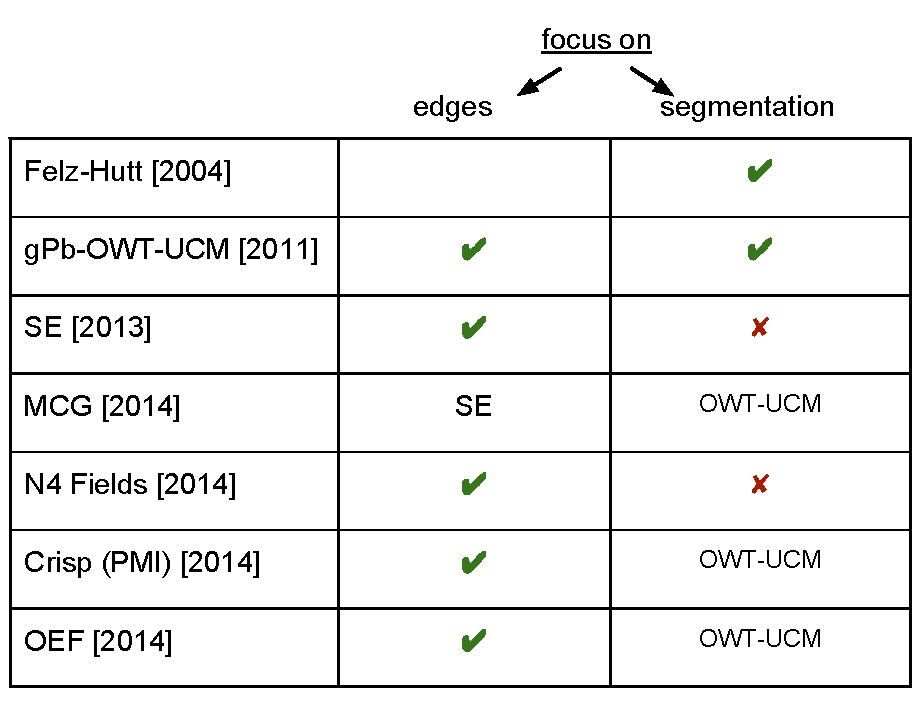
\includegraphics[width=0.8\textwidth]{images/intro/related_work_table.pdf} % OMG, that looks so much better and compiles faster (than .png); if possible, export Google drawings as pdf from now on % related_work_table.png
\caption[Related work: state of the art]{Where do state-of-the-art methods for edge detection and segmentation innovate?} %focus there efforts.}
\label{fig:related_work_table}
\end{figure}

\section{Goal}
Our objectives are  twofold:  first to provide a principled way of obtaining hierarchical image segmentation based on probabilistic edge detection results ({\it Pb}), and second, to explore ways to improve the quality of the so %thus 
obtained segmentation.
% a more principled approach to boundary-guided image segmentation. % analysis?

\section{Outline}
The rest of this work is structured as follows: 

Chapters \ref{Chapter2} and \ref{Chapter3} review two related methods that are highly relevant to our current work. 
\cref{Chapter2} describes the {\tt SE} edge detector which trains a decision forest to model the relationship between a local image patch and its segmentation. 
\cref{Chapter3} details % highlights recount discuss explain detail outline relate
the edge detector and segmentation machinery {\tt gPb-OWT-UCM}. Despite the segmentation pipeline {\tt OWT-UCM} demanding an oriented boundary signal, it is currently a widely applied post-processing step to allow edge detectors to ``close'' contours and provide segmentation. 

In \cref{Chapter4} we describe our proposed algorithm for obtaining a hierarchical segmentation from extracted edges by using only local information. Our experiments and evaluation are in \cref{Chapter5}. 

We finish in \cref{Chapter6} by summarising our findings and highlighting open questions that might be a basis for future investigation. %searchings.

